\subsection{Schwellspannung}
Mit den Szintillatoren soll minimal ionisierende Strahlung gemessen werden. Daf�r werden die Schwellen etwas unterhalb des Energieverlustes der Flach-Szintillatoren, im Bereich von 1,2MeV eingestellt. F�r die Justierung wird ein $^{60}$Co Pr�parat verwendet. Die untere Schwelle f�r den Blockdiskriminator, im Bereich von 1,5-2MeV soll m�glichst niedrig eingestellt werden, jedoch hoch genug, um den Untergrund der Praktikumsr�ume auszublenden. Dabei soll das Signal-Rausch-Verh�ltnis maximal werden. Um das Signal-Rausch-Verh�ltnis zu maximieren, wurde zuerst bei allen Diskriminatoren die Differenz zwischen dem Signal mit $^{60}$Co-Pr�parat und dem Signal ohne $^{60}$Co-Pr�parat bestimmt. Die bestimmten Schwellspannungen sind in den Abb. \ref{fig:Disk_1}, \ref{fig:Disk_2}, \ref{fig:Disk_3} und \ref{fig:Disk_4} zu sehen.
\begin{figure}[H]
\centering
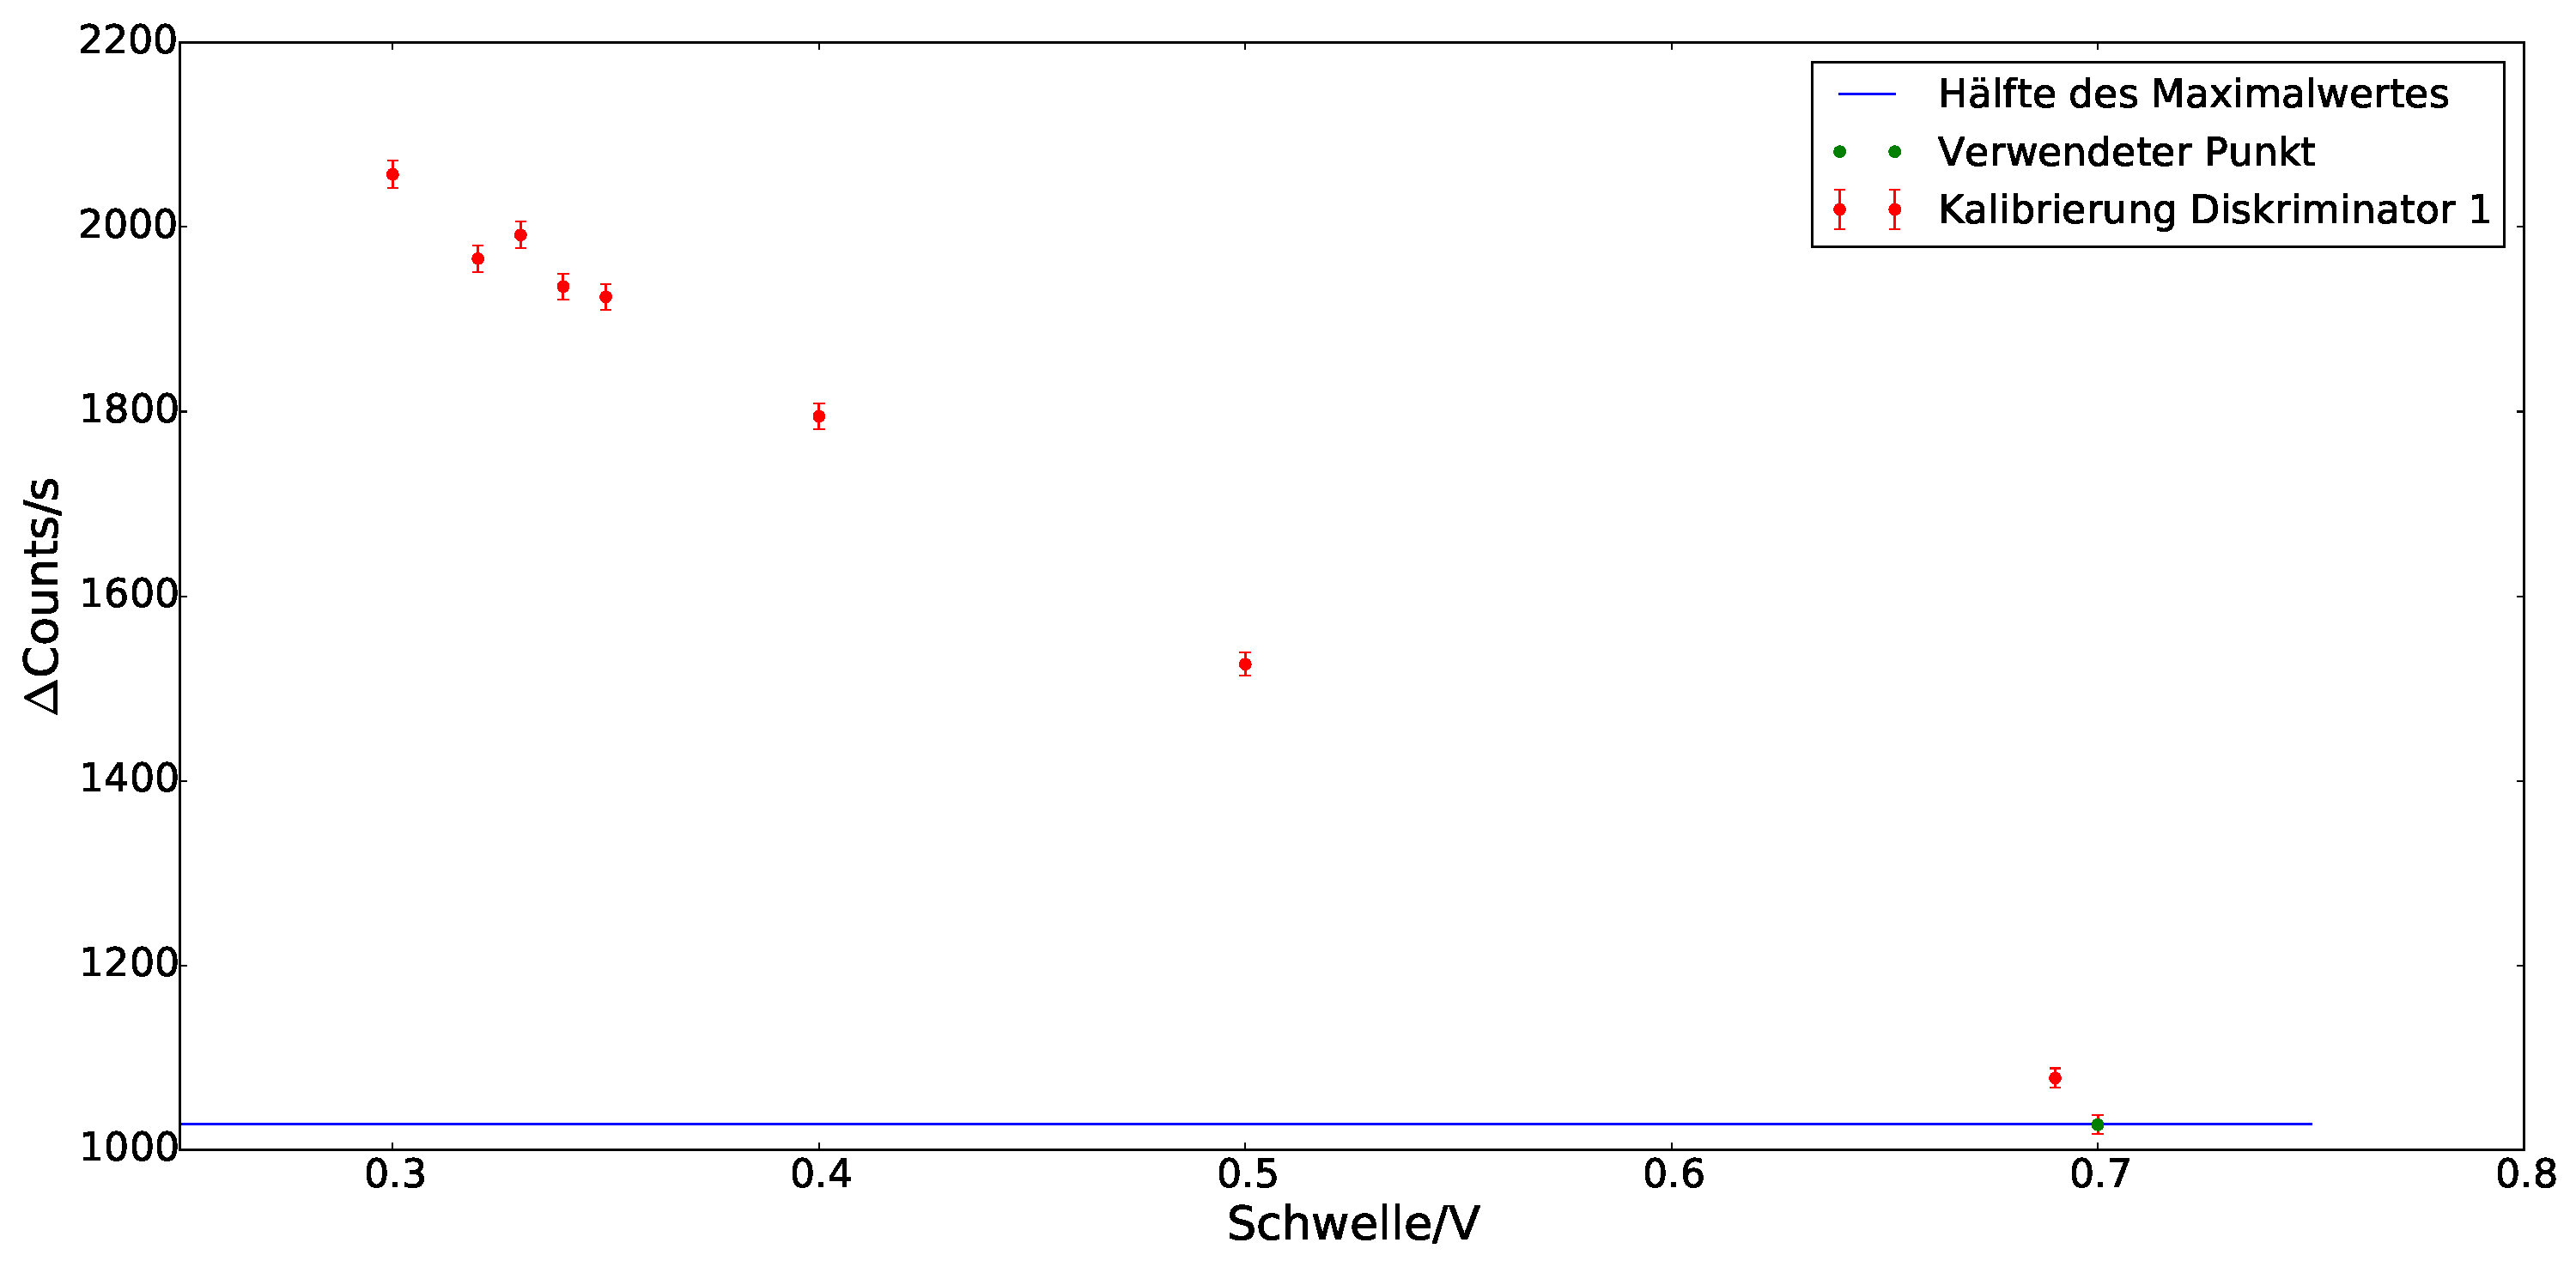
\includegraphics[scale = 0.35]{Disk_1.pdf}
\caption{Differenzplot der Counts gegen die Schwellspannung f�r Diskriminator 1}
\label{fig:Disk_1}
\end{figure}
\begin{figure}[H]
\centering
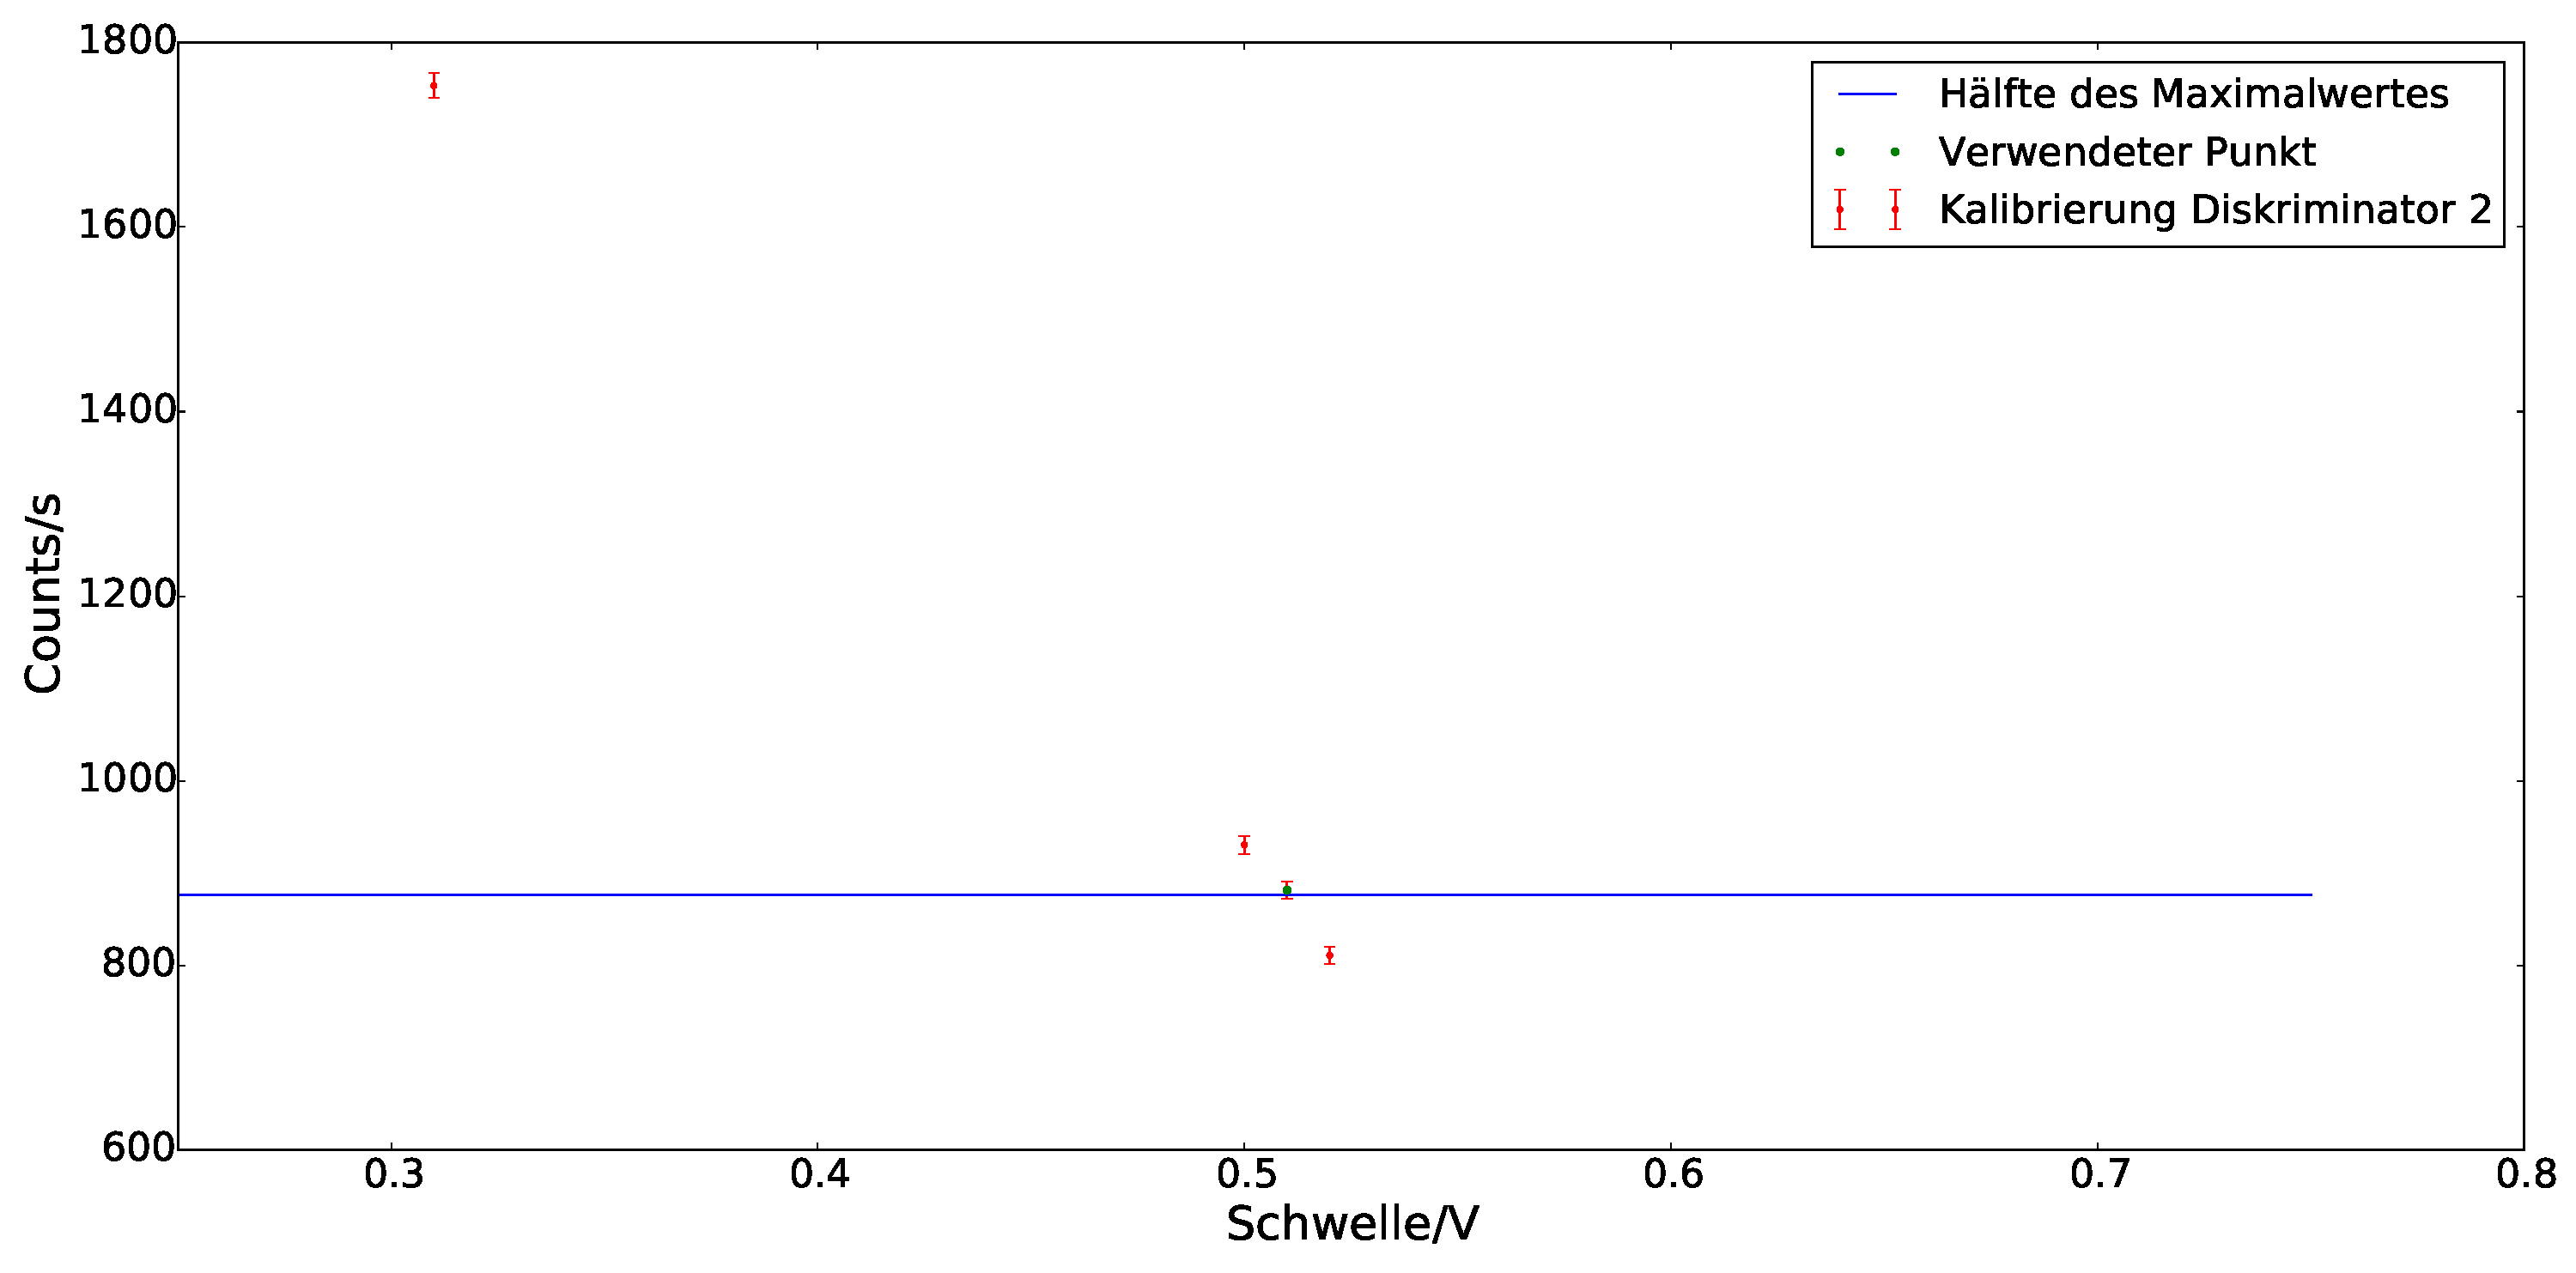
\includegraphics[scale = 0.35]{Disk_2.pdf}
\caption{Differenzplot der Counts gegen die Schwellspannung f�r Diskriminator 2}
\label{fig:Disk_2}
\end{figure}
In Abb. \ref{fig:Disk_3} wurde zus�tzlich eine etwas h�here Schwelle eingestellt, welche auf H�he des Plateaus zwischen den beiden Energien der von $^{60}$Co emittierten Photonen liegt. Nach der Einstellung des Delays, wodurch erreicht werden soll, dass die beiden oberen Szintillatoren (1 und 2) gleichzeitig mit dem 3. Szitillator triggern, wird die Diskriminatorschwelle f�r den 3. Szintillator auf den h�heren Wert gestellt, sodass dieser w�hrend der Messung nur bei Zerfall eines Myons triggert. Szintillator 1 und 2 triggern w�hrend der Messung genau beim Eintritt des Myons in Szintillator 3, wobei Szintillator 3 erst im Falle eines Zerfalls triggert (2. Diskriminatorschwelle). 
\begin{figure}[H]
\centering
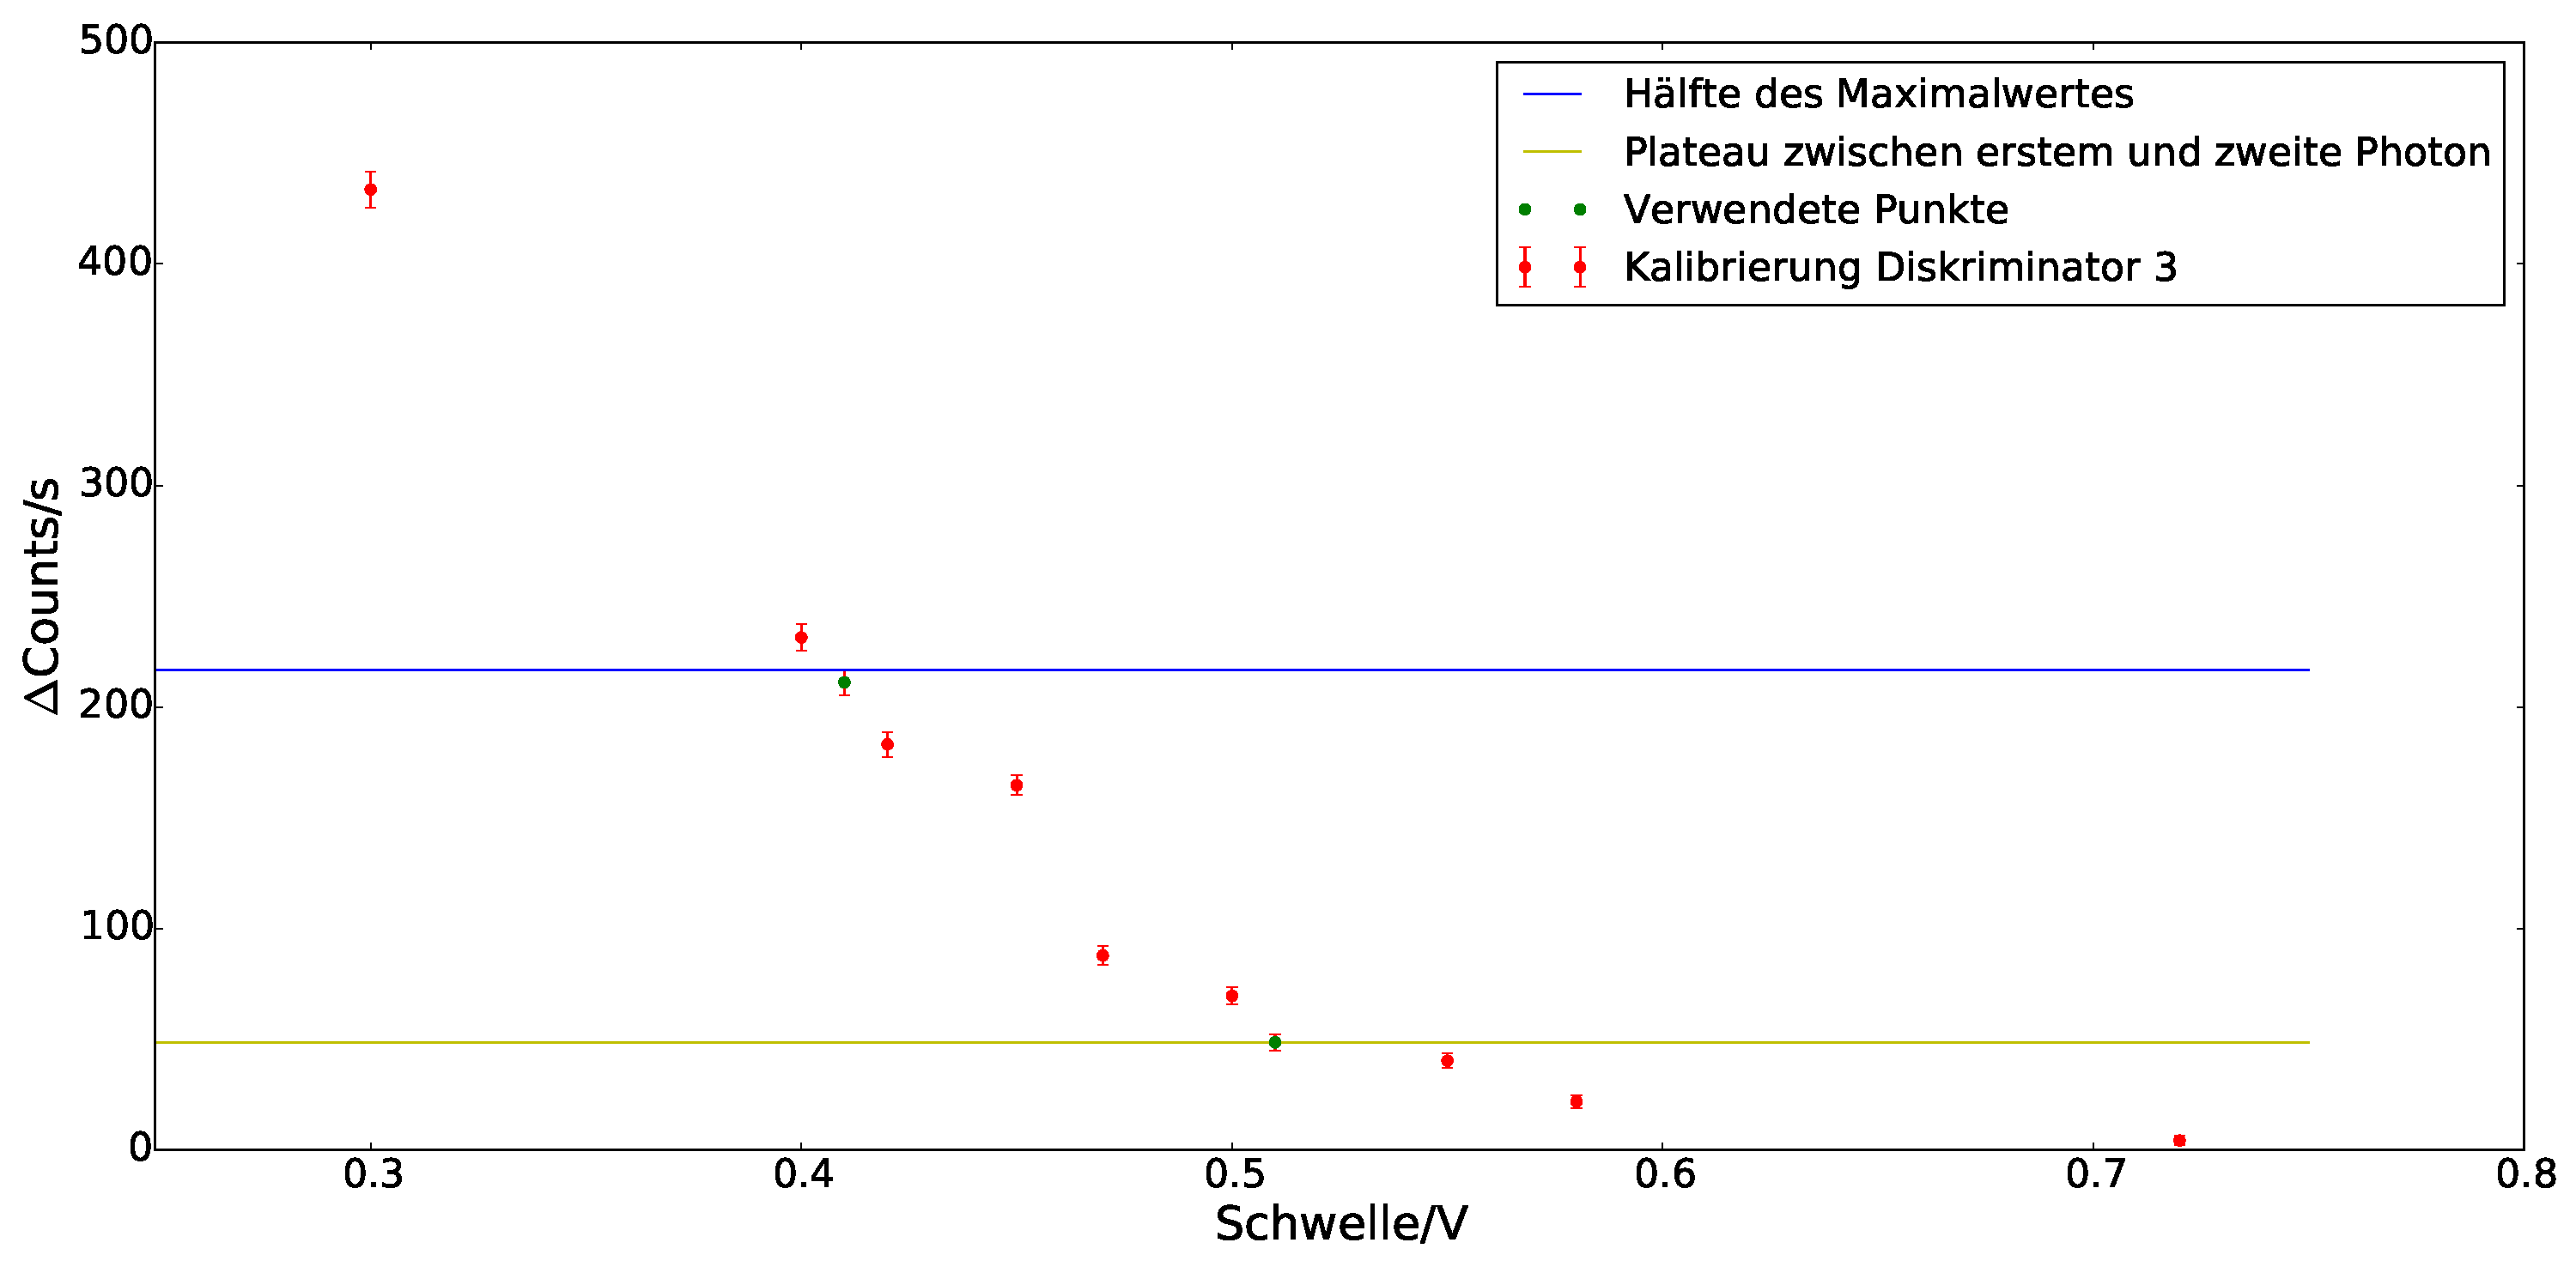
\includegraphics[scale = 0.35]{Disk_3.pdf}
\caption{Differenzplot der Counts gegen die Schwellspannung f�r Diskriminator 3}
\label{fig:Disk_3}
\end{figure}
\begin{figure}[H]
\centering
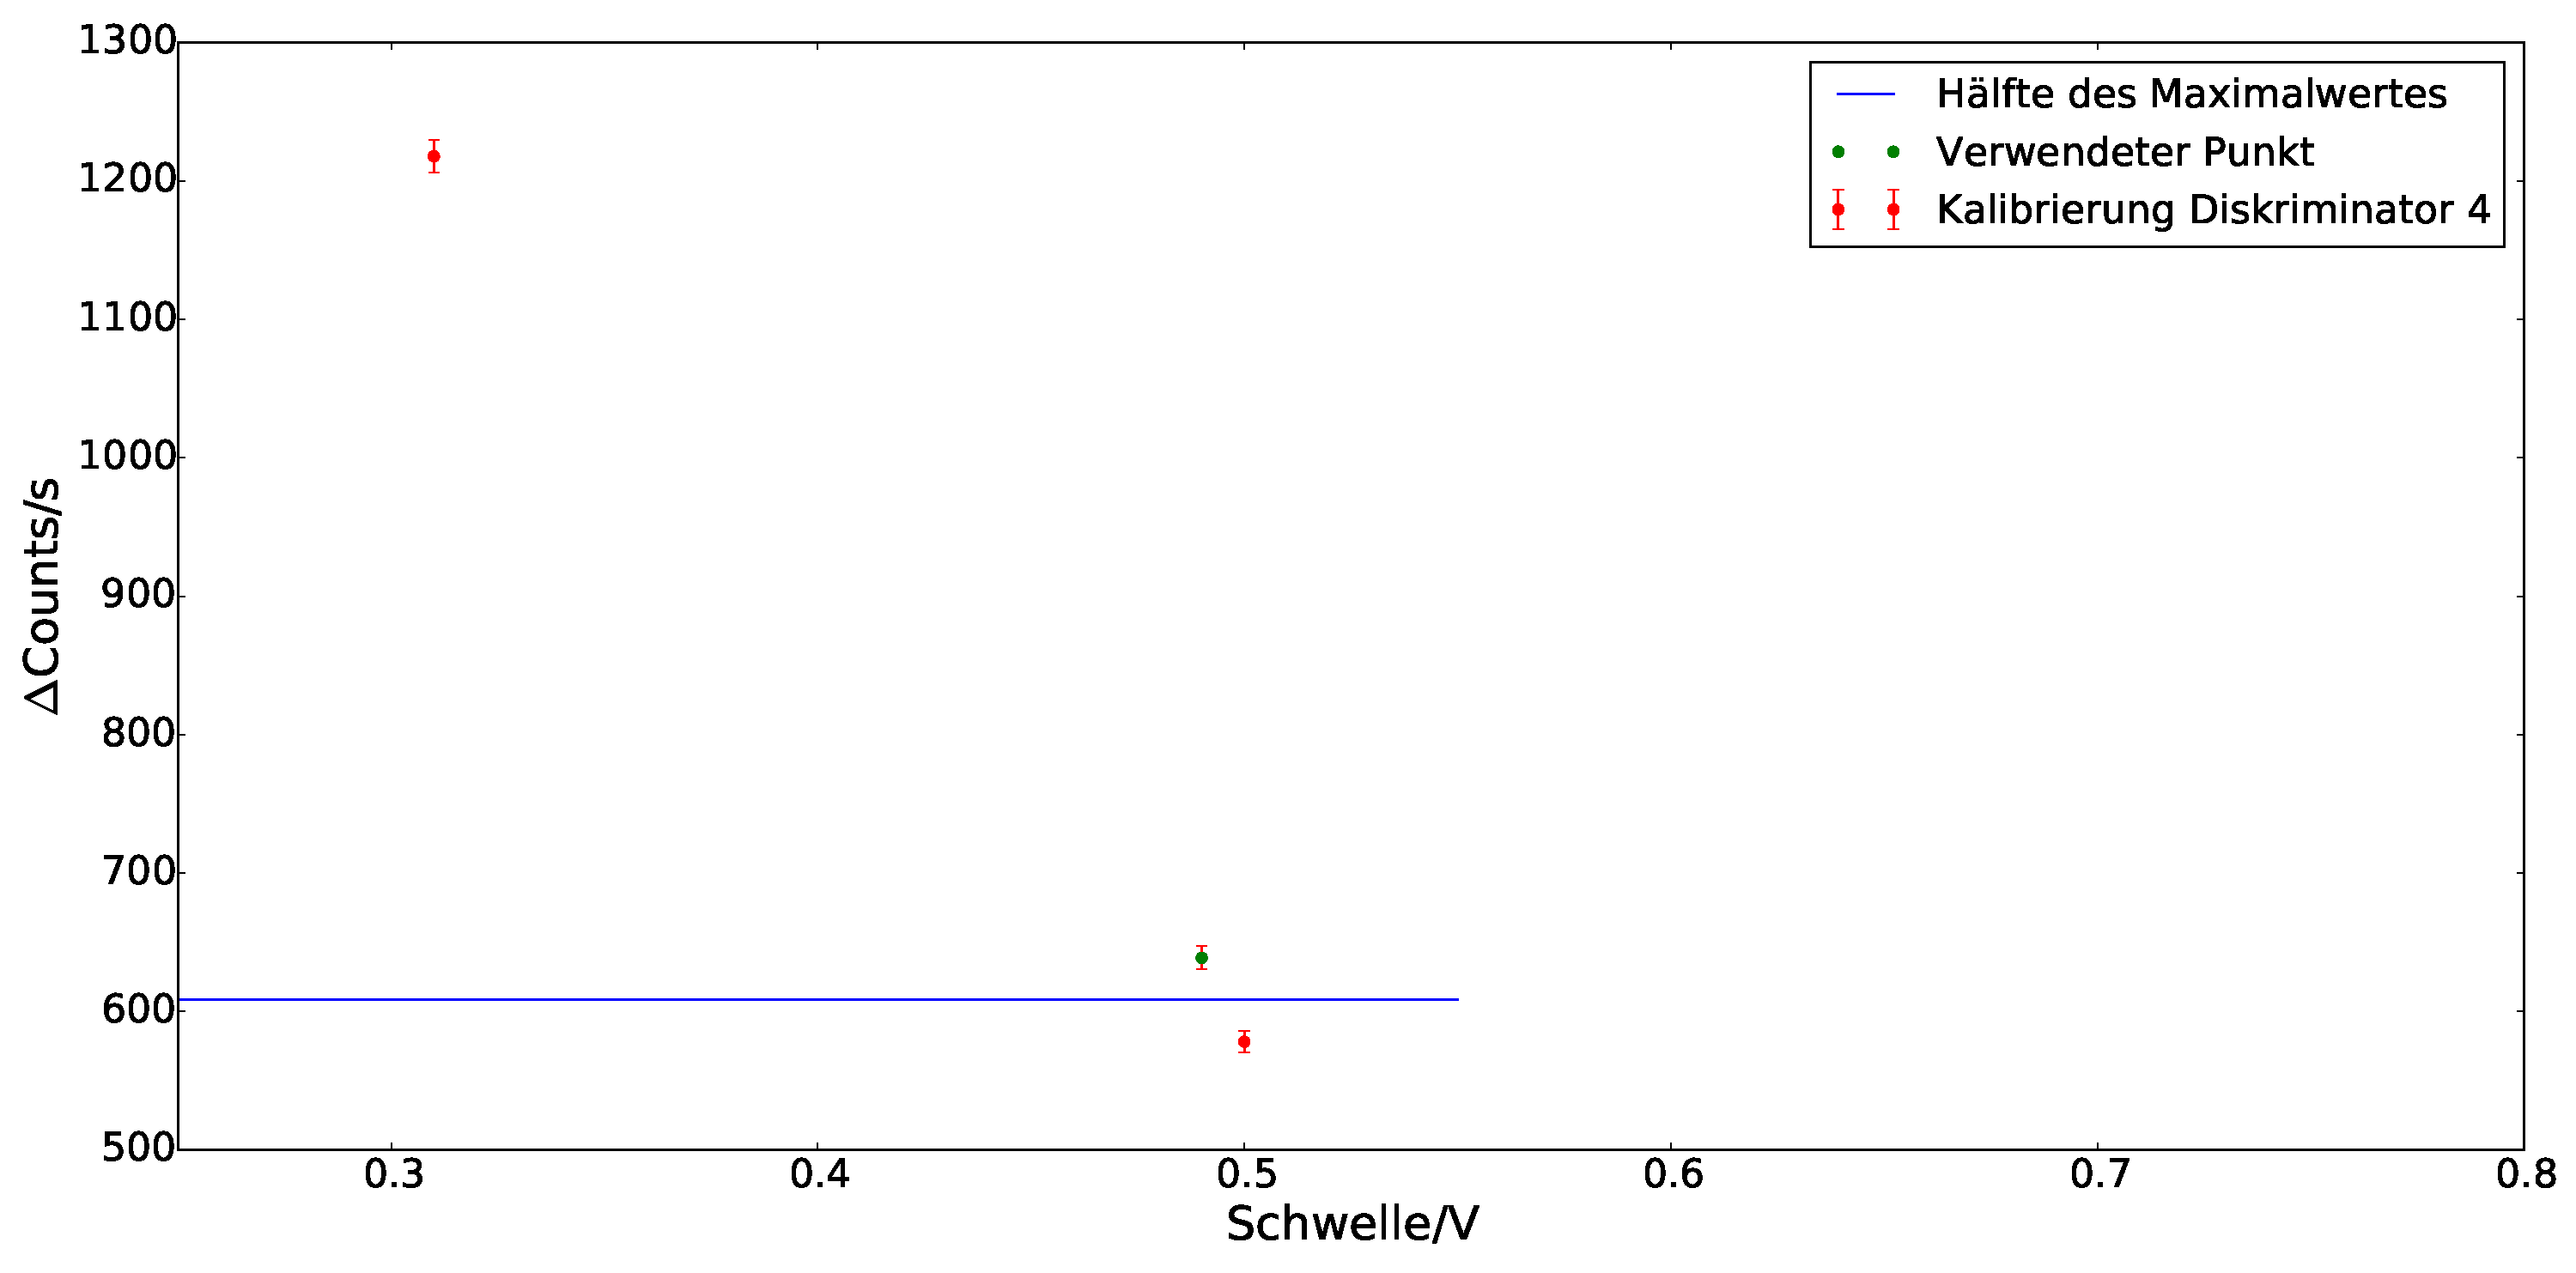
\includegraphics[scale = 0.35]{Disk_4.pdf}
\caption{Differenzplot der Counts gegen die Schwellspannung f�r Diskriminator 4}
\label{fig:Disk_4}
\end{figure}
Die Energien der Photonen beim Zerfall von $^{60}$Co werden in Abb. \ref{fig:Co_60} dargestellt.(vgl. \cite{Co_60})
\begin{figure}[H]
\centering
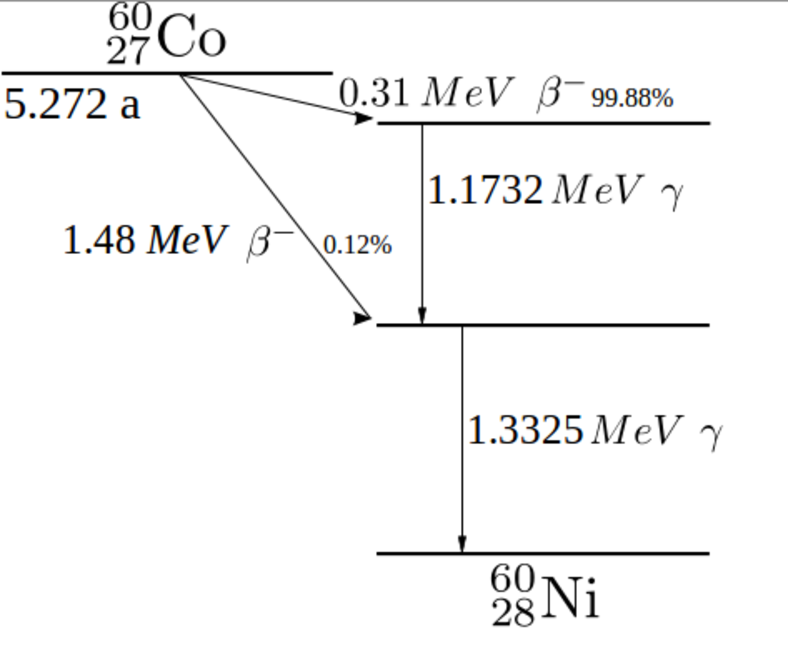
\includegraphics[trim = 0cm 0cm 0cm 1.1nm,scale = 0.5,clip]{Cobalt60_Zerfall.pdf}
\caption{Zerfall von $^{60}$Co}
\label{fig:Co_60}
\end{figure}
In Tabelle \ref{tab:Schwellwerte} sind die Diskriminatorschwellen f�r Diskriminator 1 bis 4 aufgelistet.
\begin{table}[H]
\caption{Diskriminatorschwellwerte}
\begin{tabular}{c|c|c|c|c|}
 & Diskriminator 1 & Diskriminator 2 & Diskriminator 3 & Diskriminator 4 \\ 
\hline Untere Schwelle & 0,70 V & 0,51 V & 0,41 V & 0,49 V \\ 
\hline Obere Schwelle &  &  & 0,52 V &  \\ 
\hline 
\end{tabular}
\label{tab:Schwellwerte}
\end{table}